%This is the third chapter of the dissertation

%The following command starts your chapter. If you want different titles used in your ToC and at the top of the page throughout the chapter, you can specify those values here. Since Columbia doesn't want extra information in the headers and footers, the "Top of Page Title" value won't actually appear.

\pagestyle{cu}
\graphicspath{{./Chapter3/images/}}

\chapter[The First Dark Matter Search with XENON1T][The First Dark Matter Search with XENON1T]{The First Dark Matter Search with XENON1T}

XENON1T is the third generation detector of the XENON Dark Matter Collaboration.  With a fiducial mass of over 1,000 kg, it is expected to be the most sensitive detector in the world to WIMPs.  This chapter will focus on the XENON1T Dark Matter Experiment and the results from its first WIMP search.  The first section will focus on the design of the detector and its subsystems while the second section will focus on background considerations and estimation for the detector.  The following section will focus on the general calibration of the detector followed by a section on the calibration of the detector to nuclear recoils.  Finally, we will discuss the results of the first dark matter search and its implications.


\section{The XENON1T Detector}
\label{sec:xe1t_detector}

In this section we will focus on the XENON1T detector and its individual subsystems that are needed for it to operate according to the working principle discussed in \secref{sec:lxe_tpc}.  For more details on the design and construction of the detector, please refer to \citeref{aprile2017xenon1t}.

\subsection{ Laboratori Nazionali del Gran Sasso}

 Laboratori Nazionali del Gran Sasso (LNGS)  is an Italian national laboratory located underneath the Gran Sasso mountain range in central Italy.  In order to shield from cosmogenic backgrounds, dark matter detectors, and detectors for low background experiments in general, are placed deep underground.  Even deep underground, very high energy muons are still not completely shielded and are a dangerous background source for dark matter searches because they can produce fast neutrons in the rock that could recoil in the detector.  The flux of these neutrons at different laboratorias has been measured in \citeref{mei2006muon} and a plot of the fluxes is shown in \figref{fig:neutron_flux}.
 
 To shield against these cosmogenic neutrons, the TPC is inside the center of a cylinder filled with water that is roughly ten meters in diameter and ten meters tall.  This will be the focus of \secref{sec:muon_veto}. 
 
\begin{figure}[t]
	\centering
	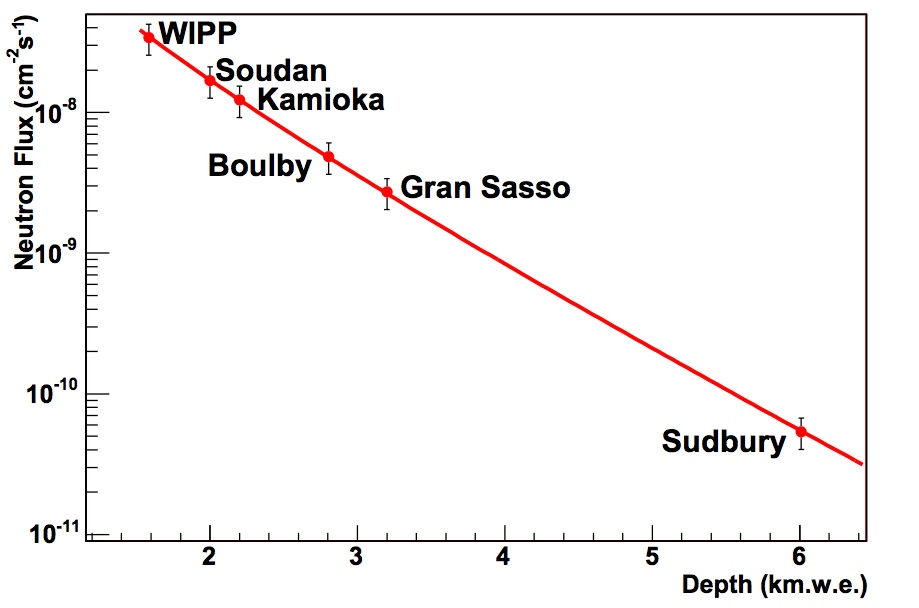
\includegraphics[width=0.8\textwidth]{neutron_flux}
	\caption{The neutron flux due to cosmogenic muons versus kilometers water equivalent depth for various underground laboratories.    Image Credit: \citeref{mei2006muon}.}
	\label{fig:neutron_flux}
\end{figure}
 
 
 \subsection{Muon Veto}
 \label{sec:muon_veto}
 
 As mentioned in the previous section, to shield against the potential cosmogenic neutron background, the TPC is placed inside of a very large water tank (~10 meter diameter and ~10 meter height).  This muon veto is outfitted with 84 8'' diameter Hamamatsu R5912ASSY high quantum efficiency PMTs to detect the light from interactions inside of the water tank and the DF2000MA reflective foil to maximize the potential measured signal \cite{aprile2014conceptual}.  A diagram showing the water tank and its PMT is shown in \figref{fig:cartoon_water_tank} and a photo of the interior of the water tank during filling is shown in \figref{fig:photo_water_tank}.  A detailed Geant4 simulation \cite{agostinelli2003geant4} of the muon events originating in the rock surrounding the laboratory shows that the efficiency of the veto is $99.78 \pm 0.05 \%$ for neutrons accompanied by the muon and $71.4 \pm 0.5 \%$ for neutrons without the initial muon.  Neutrons are accompanied by muons roughly $\sfrac{1}{3}$ \cite{aprile2014conceptual}.  
 
 
 \begin{figure}[t]
	\centering
	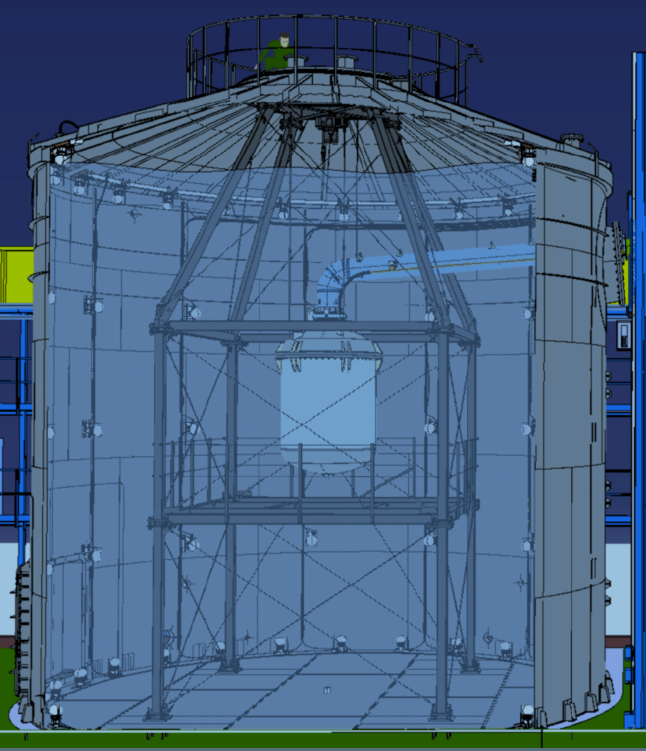
\includegraphics[width=0.6\textwidth]{cartoon_full_water_tank_muon_veto}
	\caption{A cartoon of the muon veto with the TPC centered inside the water tank.}
	\label{fig:cartoon_water_tank}
\end{figure}
 
 In addition to screening cosmogenic neutrons, the muon veto also acts as a shield to external gamma ray and neutron sources.  The neutrons mainly come from the spontaneous fission of \ce{^{238}Ur} and the \ce{^{232}Th} $(\alpha, \, n)$ reactions, both of which are found in small quantities in the surrounding rock and concrete.  Detailed Geant4 simulations \cite{agostinelli2003geant4} show that the external gamma ray background is reduced by approximately 7 orders of magnitude across 4 meters of water and the external neutron background is reduced by approximately 6 orders of magnitude per meter of water.  
 
 Given the expected fluxes for cosmogenic neutrons and radiogenic neutrons from the rock and concrete, $8.1 \cdot 10^{-10}$ above 1 MeV \cite{mei2006muon} and $8.7 \cdot 10^{-7}$ $\frac{n}{\textrm{cm}^2 \textrm{s}}$ above 1 keV, respectively, combined with the expected attenuation and cut efficiency result in a negligible external neutron background $< 0.01 \frac{\textrm{events}}{\textrm{y}}$ \cite{aprile2016physics}.
 
 
 \begin{figure}[t]
	\centering
	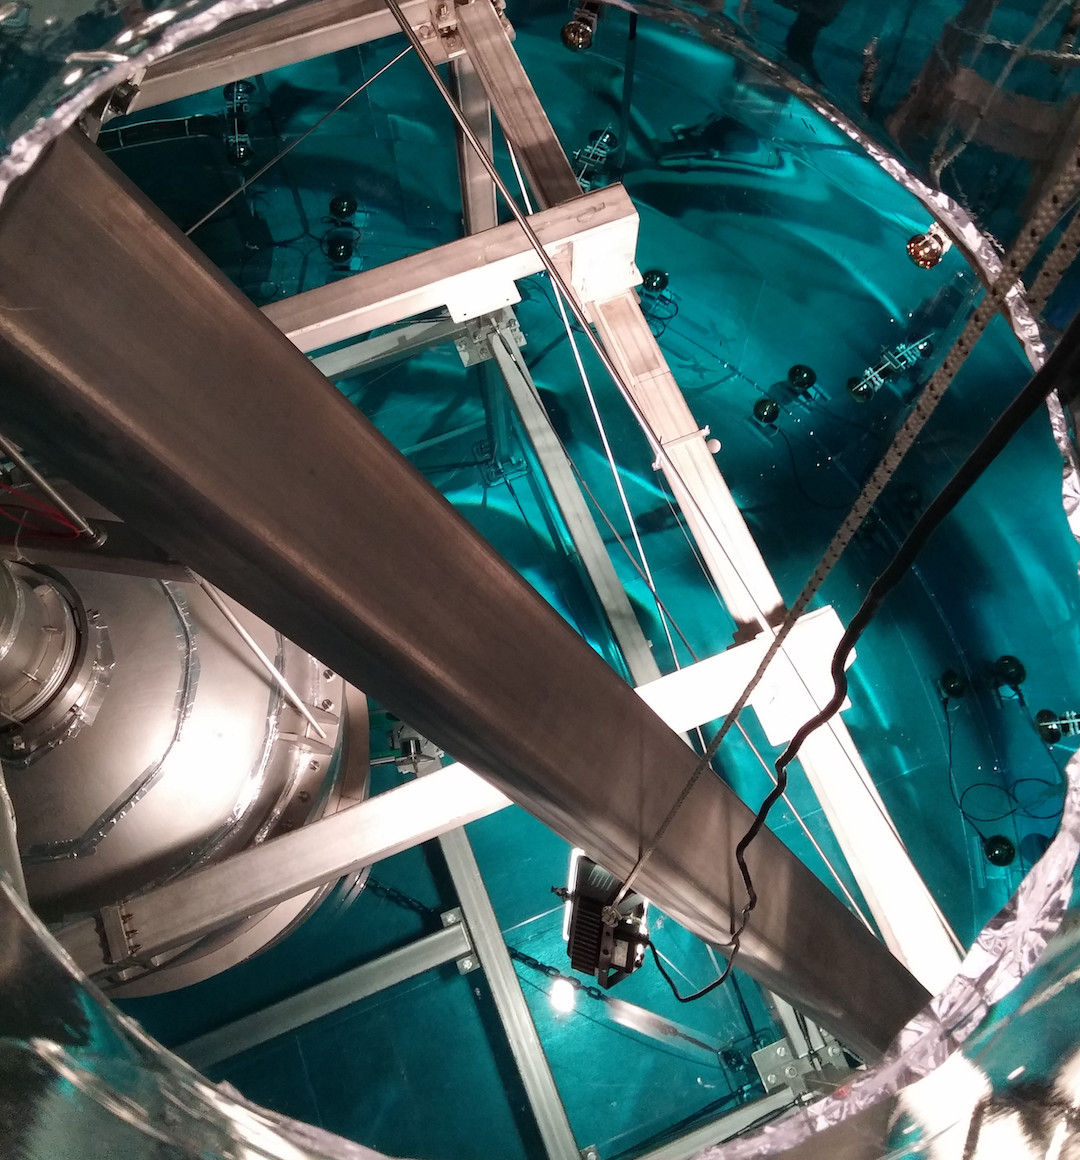
\includegraphics[width=0.6\textwidth]{water_tank_filling}
	\caption{A photo of the inside of the muon veto water tank.  The 8'' PMTs can be seen along the edges of the tank and the TPC can be seen in the center of the tank (left side of the photo).}
	\label{fig:photo_water_tank}
\end{figure}



 \subsection{Cryostat}
 \label{sec:cryostat}


In between the TPC itself and the water of the water tank is the cryostat.  The cryostat is a double-walled vacuum insulated vessel designed to contain the detector assembly and 3.5 tons of liquid xenon.  The cryostat itself is made of 5 mm thick, low radioactivity stainless steel.  The inner part of the cryostat, since it needs to house such a large amount of liquid xenon at roughly $-96^{\circ}$C, is covered in a blanket of aluminized mylar foil to minimize radiative heat transfer (shown in \figref{fig:xe1t_inner_cryostat}).  The outer cryostat is large enough to hold and support  XENON1T's inner vessel and TPC but also the inner vessel and TPC of XENONnT, a planned upgrade of XENON1T.  A diagram of the cryostat and the TPC is shown in \figref{fig:xe1t_cryostat_tpc}.

\begin{figure}[t]
	\centering
	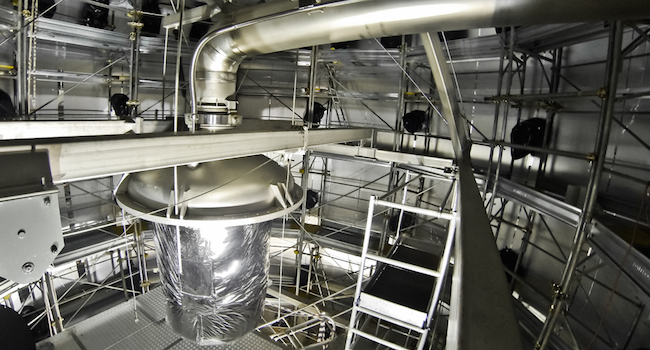
\includegraphics[width=0.99\textwidth]{xe1t_inner_cryostat}
	\caption{A photo from inside the watertank with the inner cryostat installed.  Note the mylar foil around the vessel for insulation against radiative heat transfer.}
	\label{fig:xe1t_inner_cryostat}
\end{figure}

\begin{figure}[p]
	\centering
	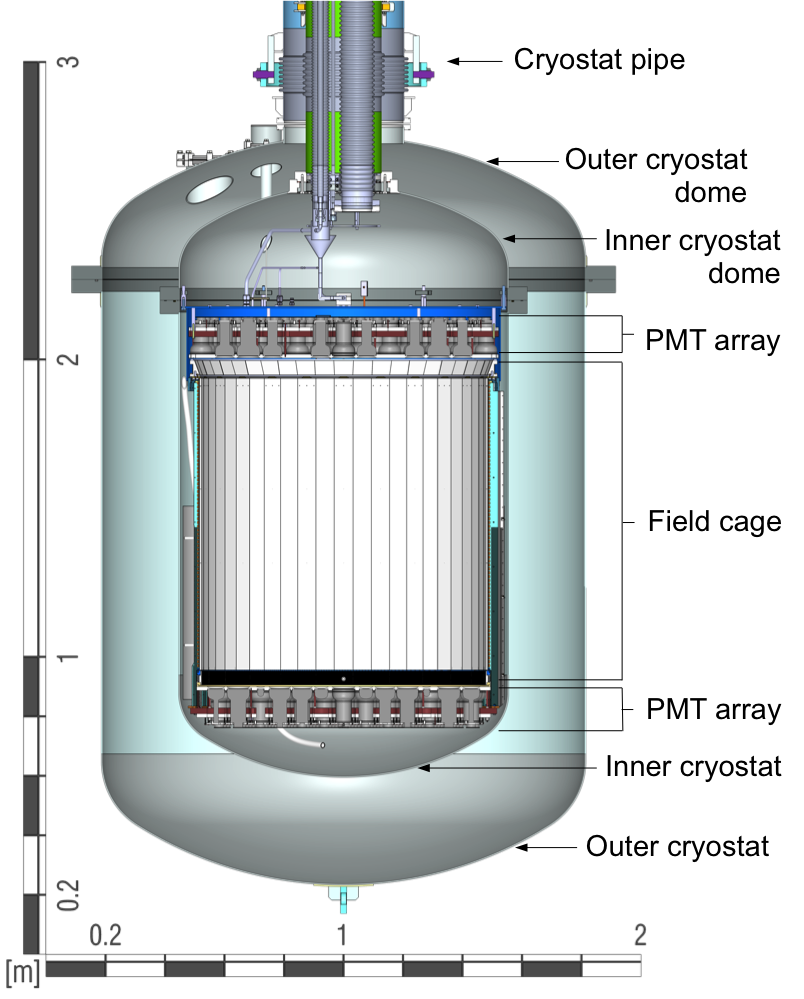
\includegraphics[width=0.99\textwidth]{xe1t_cryostat_tpc}
	\caption{A diagram of the cryostat, the TPC, and the subsystems of each.  Image Credit: \citeref{aprile2017material}.}
	\label{fig:xe1t_cryostat_tpc}
\end{figure}

The cryostat is connected to external systems such as the purification and cryogenic systems via a double-walled vacuum insulated pipe.  This pipe not only carries liquid xenon and gaseous xenon to and from the different systems but also houses the various cables that need to go into the detector (mainly signal and high voltage cables).  These cables are stored inside of a smaller pipe so that radon emanations lead away from the TPC.  One of the gaseous xenon lines is used to pressurize the xenon diving bell, which is used to set the liquid level in the detector.

The weight of the cryostat and TPC are supported by three stainless steel rods.  These rods are connected to several motion feedthroughs such that the level of the xenon in the TPC is approximately 100 $\mu$m.  These systems are also designed for XENON1T and XENONnT.

A schematic of the cryostat, TPC, and many of the subsystems that will be discussed is shown in \figref{fig:diagram_cryo_pur_sys}.


\begin{figure}[t]
	\centering
	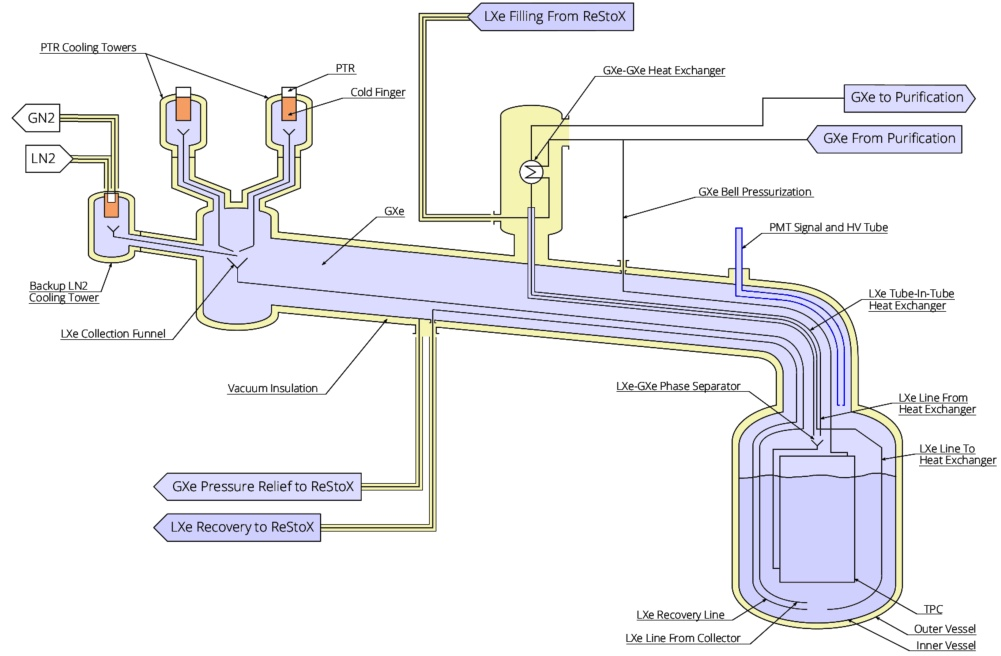
\includegraphics[width=0.99\textwidth]{diagram_cryo_pur_sys}
	\caption{A diagram of the cryostat, the cryogenics system, and the purification systems.  Image Credit: \citeref{aprile2017material}.}
	\label{fig:diagram_cryo_pur_sys}
\end{figure}


 \subsection{Cryogenics System}
 \label{sec:cryogenics_system}
 
 To keep the 3.5 tons of liquid xenon cool, two pulse tube refrigerators (Iwatani PC-150 PTRs) are used.  Each of the PTRs provides a cooling power of approximately 250 W while the estimated total heat load of the system (including the removal of electronegative impurities which will be discussed in \secref{sec:xe1t_pur_electronegative}) is less than 150 W.  Therefore, this system is doubly-redundant and designed such that a PTR can be removed and replaced during operation of the detector.  These PTRs are connected to copper cold fingers on which the gaseous xenon condensates and flows back into the detector.  The xenon pressure inside of the cryostat is controlled via resistive heaters thermally connected to the copper cold fingers.  These resistive heaters are  controlled by a proportional-integral-derivative (PID) controller that adjusts the power of the heaters to maintain a desired cold-finger temperature \cite{aprile2017xenon1t}.
 
 The photomultiplier tubes (which will be discussed in \secref{sec:photomultiplier_tubes}) are susceptible to damage if the pressure in the detector becomes too high.  For this reason, it is crucial to be able to keep the pressure stable even in the event of an emergency.  XENON1T was designed such that if there is a sudden increase in pressure, a cold finger that is cooled using liquid nitrogen is used in place of the PTRs.  To maintain normal operating conditions in the detector only ~100 liters per day are required (the tank containing liquid nitrogen can store up to 10 $\textrm{m}^3$) \cite{aprile2017xenon1t}.
 
 The three redundant cooling systems can be seen on the left side of \figref{fig:diagram_cryo_pur_sys}.  The gas in the pipe condenses on the cold fingers and then is fed back into the cryostat.

 
 \subsection{Purification Systems}
 \label{sec:xe1t_pur}
 
 There are two main purification systems in XENON1T: one for electronegative impurities and a second for the removal of \ce{^{85}Kr}.  
 
 \subsubsection{Electronegative Impurities}
 \label{sec:xe1t_pur_electronegative}
 
 As mentioned in \secref{sec:tpc_s2_sig}, electronegative impurities, mainly oxygen, enter the liquid xenon through the various materials used when constructing the detector.  These electronegative impurities can capture free electrons that are drifted to produce the secondary signal, the S2.  This causes a complete loss of signal in the case of high concentrations but will still causes large smearing effects at low levels of concentration (ppb levels of \ce{O_2} relative to xenon), reducing the discrimination power of liquid xenon for electronic and nuclear recoils.
 
Materials are cleaned before being installed in the detector however these electronegative impurities are constantly outgassing into the detector and therefore the xenon must be constantly cleaned.  To achieve high purity, a doubly redundant purification system that is connected to the cryostat is used (center of \figref{fig:diagram_cryo_pur_sys}).  This system includes two loops with a gas driving pump (CHART QDrive) and a high-termperature arare-gas purifier (SAES PS4-MT50-R getter) \cite{aprile2017xenon1t}.  The SAES getter is able to reduce the \ce{O_2}, \ce{H_2O}, \ce{CO}, \ce{CO_2}, \ce{H_2}, \ce{N_2}, and \ce{CH_4} concentrations to low ppb or below by having the impurities form irreveersible chemical bonds with the material inside of the getter.  One drawback of the getter is that it must be operated at high temperatures ($\sim 50^{\circ} \, \textrm{C}$).  However, this effect can be reduced by using heat exchangers between both the hot and cold liquid and gaseous xenon.  The gaseous heat exchanger can be seen in the center of  \figref{fig:diagram_cryo_pur_sys} and the liquid heat exchanger (tube-in-tube) can be seen on the right side of \figref{fig:diagram_cryo_pur_sys}.  These heat exchangers are approximately 96\% efficiency and significantly reduce the heat input of the getters to 0.39 $\sfrac{\textrm{W}}{\textrm{SLPM}}$ \cite{aprile2017xenon1t}.

% getter specs: http://www.saespuregas.com/Library/specifications-brochures/s110-233_a_521.pdf
 
 
 \subsubsection{\ce{^{85}Kr}}
 
 A cryogenic distillation column is used to reduce the natural krypton to xenon level to below 200 ppq (part per quadrillion).  The cryogenic distillation column leverages the different vapor pressures of the two elements around the xenon boiling point: the vapor pressure of krypton is roughly 10.8 times higher than the vapor pressure of xenon at 175 K and 2 bars.  For a dual-phase system in equilibrium, this implies that the gaseous phase will be enriched with krypton relative to the liquid by this factor of 10.8 --- this simple dual-phase system is referred to as a single distillation stage.  To improve this separation efficiency, one can put several of these distillation stages in series with each other.  This multi-stage distillation column can practically be achieved via a package material that replicates these additional stages when placed inside of a single stage.  The height of the material ultimately translates into the number of stages added \cite{fieguth2016distillation}.
 
 The concentration can be measured with an RGMS (residual gas mass spectrometer) or an RGA (residual gas analyzer).  A distillation column with 2.8 meters of the Sulzer EX package material was deployed for XENON1T and achieved natural krypton to xenon levels of $< 48$ ppq \cite{aprile2017removing}.  
 
 A similar distillation column was also built to test the possibility of radon removal.  Using 1 meter of package material, a radon reduction factor of $>$ 27 was achieved \cite{aprile2017online}.
 
 
  \subsection{Recovery and Storage}
 
 For small detectors, it sufficed to fill detectors via cooling the xenon stored in bottles and to empty the detector by evaporating the liquid xenon.  While simple, this method is inefficient and would require approximately 250 W of heating power over 2 months to fill the XENON1T detector \cite{aprile2017xenon1t}.  While an emergency situation is unlikely in XENON1T due to its many redundancies, this simple method would also make recovery of all of the xenon very difficult.
 
 Instead of storing unused xenon in bottles kept at room temperature, a new approach to recovery and storage of xenon was applied: a single 5 cubic meter vacuum-insulated stainless steel sphere rated for pressures up to 73 bar was built for this purpose, appropriately name RESToX (recovery and storage of xenon).  Similar to the detector's cryostat, several layers of aluminized mylar blanket the inner wall of this system such that the heat load on this system is only roughly 50 W.  RESToX is cooled using 16 liquid nitrogen lines that are welded to the outside of the inner wall.  To assure that the xenon inside of RESToX is kept at a precise temperature and pressure (to avoid freezing), a heating system has also been installed in the center of the vessel.
 
 RESToX is directly connected to the cryostat for filling and recuperation of the xenon gas as well as both purification systems such that the xenon stored can be kept clean and ready for use.  Xenon can be transferred into the cryostat via the pumps of the purification system (up to a maximum speed of 50 SLPM). Xenon is transferred from the cryostat to RESToX solely due to the pressure difference between the two systems.
 
 \begin{figure}[t]
	\centering
	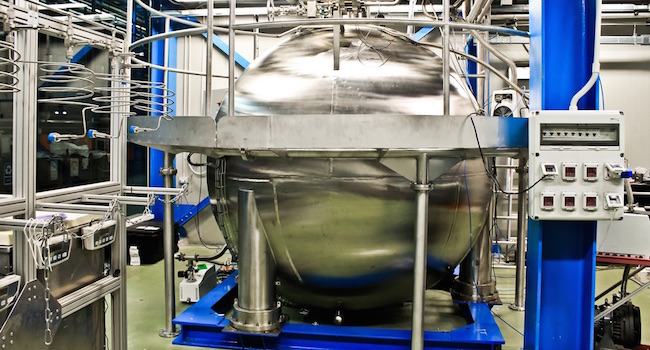
\includegraphics[width=0.99\textwidth]{xe1t_restox}
	\caption{A photograph of RESToX prior to instillation at LNGS.}
	\label{fig:xe1t_restox}
\end{figure}


  \subsection{Calibration Systems}
 \label{sec:xe1t_calibration_system}
 
While, like LUX \cite{akerib201783}, internal sources, such as \ce{^{83m}Kr}, can be injected through the purification system, a new method for introducing external sources needed to be developed due to the massive water tank surrounding the TPC.  The solution was the installation of two belts that could be used to move external sources around the bottom of the detector (the ``U-Belt'') and along the sides of the detector (the ``I-Belt'') and an additional mechanism to move the neutron generator vertically along the side of the TPC.  The main external sources used are \ce{^{228}Th} (which has several $\gamma$ lines between 511 -- 2,614 keV), \ce{^{137}Cs} (which has a single $\gamma$ line at 662 keV), and AmBe (which produces MeV energy neutrons).  The neutron generator (NSD Gradel Fusion NSD-35-DD-C-W-S) uses the deuterium-deuterium fusion process to create neutrons with energies between 2.2 and 2.7 MeV.  This generator has been specially designed to provide very low neutron rates ($\mathcal{O} \left(10 \, \sfrac{\textrm{n}}{\textrm{s}} \right)$) as well as high neutron rates ($\mathcal{O} \left(10^6 \, \sfrac{\textrm{n}}{\textrm{s}} \right)$).  These external source systems are shown in \figref{fig:xe1t_external_sources}.

Like previous generations of detectors, the PMTs are calibrated using pulsed blue light fed into the detector by fiber optic cables.  In XENON1T, four such fiber optic cables are fed into the detector at different heights and positions.


 \begin{figure}[t]
	\centering
	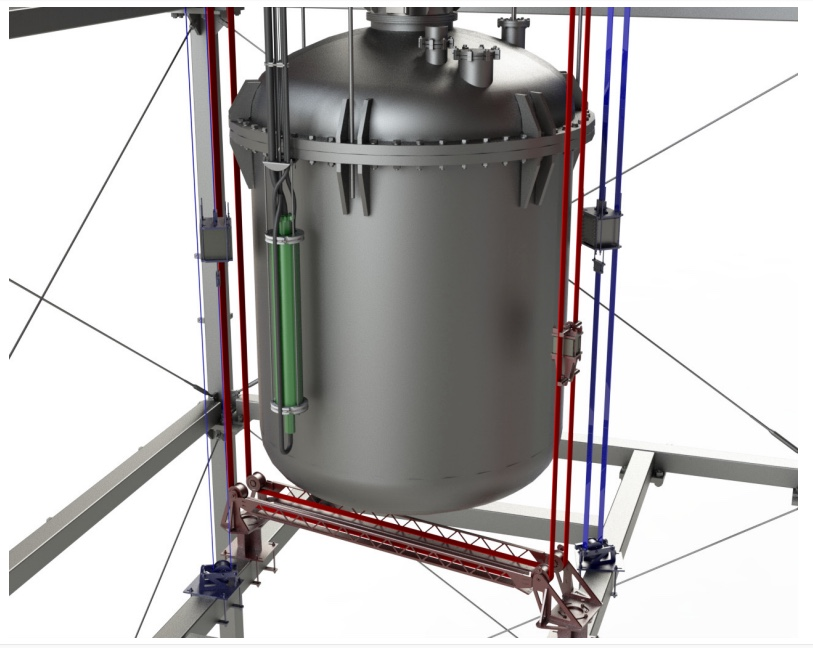
\includegraphics[width=0.7\textwidth]{xe1t_external_sources}
	\caption{A diagram showing the external calibration systems.  The ``U-Belt'', which allows for placement of external sources below the TPC, is shown in red while the ``I-Belt'', which allows for the placement of external sources at different heights along the side of the TPC, is shown in blue.  Shown in green is the neutron generator which can be raised an lowered along the side of the detector.}
	\label{fig:xe1t_external_sources}
\end{figure}
 
 
 \subsection{Photomultiplier Tubes}
 \label{sec:photomultiplier_tubes}
 
XENON1T utilizes a total of 248 high quantum efficiency  R11410-21 3 inch PMTs --- 127 of these PMTs are located in the top array and the remaining 121  are located in the bottom array.  The R11410-21 was specifically designed for XENON1T to have a high quantum efficiency, high collection efficiency, low radioactivity, and operate stably at liquid xenon temperatures.  

321 of the R11410-21 PMTs were tested for quantum efficiency, dark rate, stability, and single photoelectron response.  Of the 321 PMTs, 78 were rejected: 12 due to high or unstable dark count rate and 53 due to after-pulsing (44 of which were confirmed to have a leak).  The PMTs were found to have an average quantum efficiency of $34.5 \pm 2.8 \%$ at 178 nm and a collection efficiency of $90 - 95 \%$ \cite{barrow2017qualification}.  PMTs that were found to have a higher quantum efficiency and collection efficiency were placed in the center to maximize potential light collection as shown in \figref{fig:xe1t_pmt_qe}.  The bottom PMT array sees the majority ($\sim 90\%$) of the light for S1s due to the reflection of light at the liquid-gas interface --- therefore, the higher quantum efficiency PMTs were placed in the bottom array.

\begin{figure}[t]
	\centering
	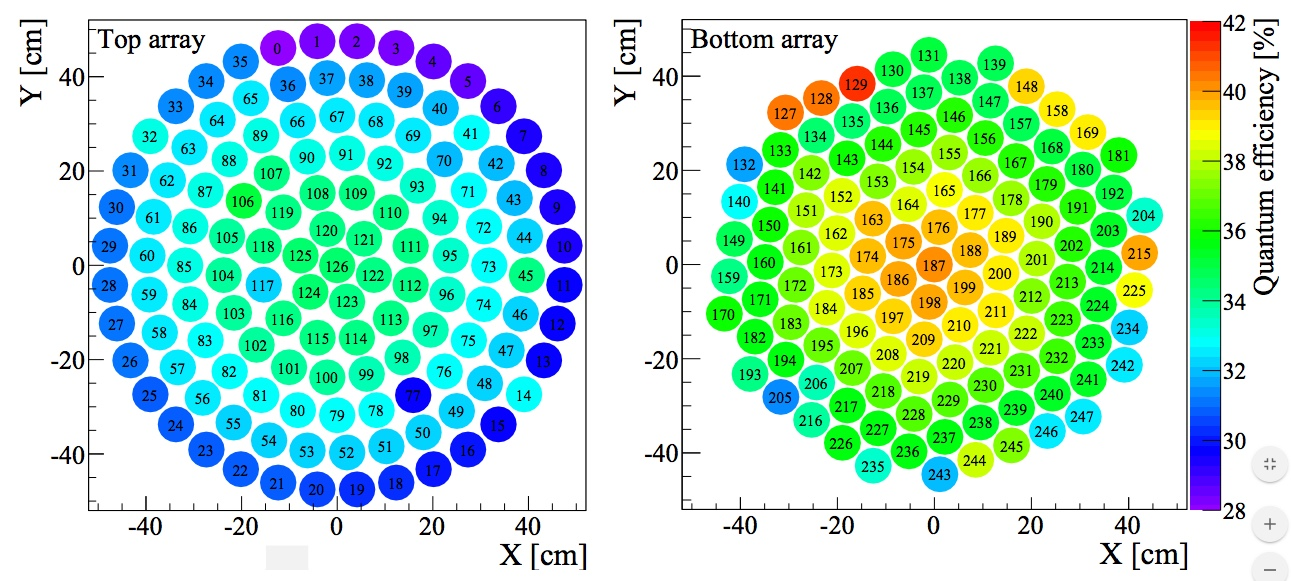
\includegraphics[width=0.99\textwidth]{xe1t_pmt_qe}
	\caption{The quantum efficiencies of the PMTs installed in the XENON1T PMT arrays.  Note that, with a few exceptions due to higher radioactivity levels, the highest quantum efficiency PMTs are placed towards the center to maximize light collection.  Also note that in general the PMTs used in the bottom array have a higher quantum efficiency than those in the top array since the much smaller S1 signal is mainly seen by the bottom array.  Image Credit: \citeref{aprile2017xenon1t}.}
	\label{fig:xe1t_pmt_qe}
\end{figure}
 
 Of the 248 PMTs installed, only 213 could be used for the first science run of XENON1T.  The reasons for omission in the final analysis varied from high levels of noise, frequent trips and flashing, and low single photoelectron acceptance at the trigger threshold.  The remaining PMTs were set such that they had a gain from $2- 5 \cdot 10^6 \, \textrm{e}^-$ and a resolution of approximately 30\%.  The gains of individual PMTs were stable over the course of data taking.
 
 % mention work on characterization of PMTs in later chapter
 
  \subsection{XENON1T TPC}
 \label{sec:xe1t_tpc}

The XENON1T has a cylindrical shape with a diameter of 96 cm and height of 97 cm at room temperature.  The TPC outer wall is made of PTFE (polytetrafluoroethylene), otherwise known as teflon.  Teflon is chosen for several reasons: it has a high reflectivity, it can be made such that it is highly radio-pure, it has low outgassing rates, it is chemically inert (so no special considerations need to be made for handling or storage), and it is an excellent insulator \cite{neves2017measurement}.  Teflon does have a high thermal coefficient of expansion resulting in a length contraction of approximately 1.4\% from room temperature to liquid xenon temperatures \cite{kirby1956thermal}.

Throughout this and second half of the previous chapter, it has been assumed that one can provide a uniform drift field in the TPC in order to extract the electrons from the interaction site to the liquid-gas interface and a uniform extraction field to extract the electrons from the liquid into the gas for amplification.  Ideally, one would use sets of parallel plates to create these uniform fields however this has the obvious drawback of not allowing for the detection of light.  Instead, the plates are replaced with ultrafine grids that can approximate a uniform field while keeping a high transparency ($\gtrapprox 90 \%$ from optical simulations).  The width of the wires used in the grids is $\mathcal{O}(0.2 \, \textrm{mm})$ and the size of the cells in the grid is $\mathcal{O}(5 \, \textrm{mm})$.  To create the two fields mentioned, the drift and extraction fields, we need three meshes: the cathode mesh ($\mathcal{O}(10-100 \, \textrm{kV})$), the gate mesh (ground), and the anode mesh ($\mathcal{O}(5 \, \textrm{kV})$).  To protect the PMTs from the high electric field, screening meshes kept at similar voltages to the PMTs ($\sim -1.5$ kV) are also installed.  To reduce edge effects and keep the field as uniform as possible out to the edge of the TPC, 74 field shaping rings made of oxygen-free high thermal conductivity copper are installed between the cathode and the anode via a chain of 5 G$\Omega$ resistors \cite{aprile2017xenon1t}.  Shown in \figref{fig:xe1t_sr0_field_sim} are the field simulations made using the final detector design and the voltages used during the first science run of XENON1T ($V_c = -12 \, \textrm{kV} \textrm{ and } V_a = 4 \, \textrm{kV}$).  

% cathode:12 kV in SR0
% anode: 4 kV
% screening: -1.55 kV (top and bottom)


\begin{figure}[t]
	\centering
	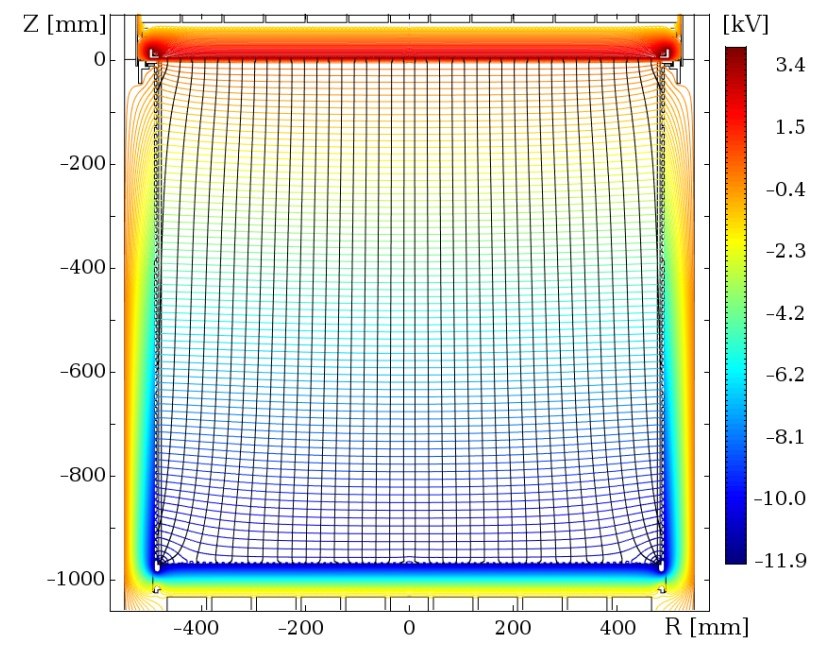
\includegraphics[width=0.99\textwidth]{xe1t_sr0_field_sim}
	\caption{The field simulations for the TPC during the first science run of XENON1T.  During this run, a cathode voltage of $-12$ kV was used and an anode voltage of $+4$ kV was used.  Image Credit: \citeref{aprile2017xenon1t}.}
	\label{fig:xe1t_sr0_field_sim}
\end{figure}


